\section{Introduction} \label{sec:csinto}

This chapter discusses Compressive Sensing \gls{cs}: an alternative signal acquisition method to Nyquist sampling, which is capable of accurate sensing at rates well below those predicted by the Nyquist theorem. This strategy hinges on using the structure of a signal, and the fact that many signals we are interested in can be compressed successfully. Thus, Compressive Sensing acquires the most informative parts of a signal directly. 

The first section surveys the mathematical foundation of CS. It covers the Restricted Isometry Property and Stable Embeddings - necessary and sufficient conditions on which a signal can be successfully acquired. Informally, these conditions suggest that the sensing operator preserves pairwise distances between points when projected to a (relatively) low dimensional space from a high dimensional space. We then discuss which operators satisfy this condition, and why. In particular, random ensembles such as the Bernoulli/Gaussian ensembles satisfy this property - we discuss how this can be applied to the problem of wideband spectrum sensing. We also survey a small amount of the theory of Wishart matrices.

The section concludes with an overview of reconstruction algorithms for CS - methods for unpacking the original signal from its compressed representation. We give insight into the minimum number of samples for reconstruction. We survey convex, greedy,and Bayesian approaches; as well as algorithms which are blends of all three. The choice of algorithm is affected by the amount of undersampling required for system performance, the complexity of the algorithm itself, and the desired reconstruction accuracy. In general: the more complex the algorithm, the better the reconstruction accuracy. The allowable undersampling depends upon the signal itself, and the prior knowledge available to the algorithm. Greedy algorithms are the simplest class, making locally optimal updates within a predefined dictionary of signal atoms. Greedy algorithms have relatively poor performance, yet are the fastest algorithms. Convex algorithms are the next most complex, based upon minimising a global functional of the signal. This class is based upon generalised gradient descent, and has no fixed number of steps. Finally Bayesian algorithms are the slowest and most complex, but offer the best performance - both in terms of undersampling (as these algorithms incorporate prior knowledge in an elegant way), and in terms of reconstruction accuracy. 

We survey some distributed approaches to compressive sensing, in particular some models of joint sparsity, and joint sparsity with innovations.

Finally, we survey some of the approaches to wideband spectrum sensing based upon compressive sensing. In particular we survey the Random Demodulator and the Modulated Wideband converter. Both of these systems make use of low frequency chipping sequences (also used in spread spectrum communication systems). These low frequency sequences provide the basis for CS - several different sequences each convoluted with the signal are sufficient to accurately sense the signal. 

\section{Preliminaries}  \label{sec:prelims}

Compressive sensing is a modern signal acquisition technique in which randomness is used as an effective sampling strategy. This is contrast to traditional, or Nyquist, sampling, which requires that a signal is sampled at regular intervals. The motivation for this new method comes from two disparate sources: data compression, and sampling hardware design. 

The work of Shannon, Nyquist and Whittaker \cite{unser2000sampling,} has been an extraordinary success - digital signal processing enables the creation of sensing systems which are cheaper, more flexible, and which offer superior performance to their analogue counterparts. For example, radio dongles, such as those which support the RTLSDR standard, which can process millions of samples per second can now be bought for as little as £12. However, the sampling rates underpinning these advances have a doubling time of roughly 6 years - this is due to physical limitations in Analogue to Digital conversion hardware. Specifically, these devices will always be limited in bandwidth and dynamic range (number of bits), whilst applications are creating a deluge of data to be processed downstream.

Data compression means that in practice many signals encountered 'in the wild' can be fully specified by much fewer bits than required by the Nyquist sampling theorem. This is either a natural property of the signals, for example images have large areas of similar pixels, or as a conscious design choice, as with training sequences in communication transmissions. These signals are not statistically white, and so these signals may be compressed (to save on storage). For example, lossy image compression algorithms can reduce the size of a stored image to about 1\% of the size required by Nyquist sampling. In fact the JPEG standard uses Wavelets to exploit the inter-pixel redundancy of images.

Whilst this vein of research has been extraordinarily successful, it poses the question: if the reconstruction algorithm is able to reconstruct the signal from this compressed representation, why collect all the data in the first place, when most of the information can be thrown away? 

Compressed Sensing answers these questions, by way of providing an alternative signal acquisition method to the Nyquist theorem. Specifically, situations are considered where fewer samples are collected than traditional sensing schemes. That is, in contrast to Nyquist sampling, Compressive Sensing is a method of measuring the informative parts of a signal directly without acquiring unessential information at the same time. 

These ideas have not come out of the ether recently however. Prony, in 1795, \cite{prony1795essai}, proposed a method for estimating the parameters of a number of exponentials corrupted by noise. This work was extended by Caratheodory in 1907 \cite{Caratheodory1907}, who proposed in the 1900s a method for estimating a linear combination of \(k\) sinusoids for the state at time \(0\) and any other \(2k\) points. In the 1970's Geophysicists proposed minimising the \(\ell_1\) norm to reconstruct the structure of the earth from seismic measurements. Clarebuot and Muir proposed in 1973, \cite{claerbout1973robust}, using the \(\ell_1\) norm as an alternative to Least squares. Whilst Taylor, Banks and McCoy show in \cite{taylor1979deconvolution} how to use the \(ell_1\) norm to deconvolve spike trains (used for reconstructing layers in the earth). Santosa and Symes in \cite{Santosa1986} introduced the constrained \(\ell_1\) program to perform the inversion of band-limited reflection seismograms. The  innovation of \gls{cs} is to tells us under which circumstances these problems are tractable.

The key insight in CS, is that for signals which are sparse or  compressible - signals which are non-zero at only fraction of the indices over which they are supported, or signals which can be described by relatively fewer bits than the representation they are traditionally captured in - may be measured in a non-adaptive way through a measurement system which is orthogonal to the signal's domain. 

Examples of sparse signals are: 

\begin{enumerate}
\item  A sine wave at frequency \(\omega\) is defined as a single spike in the frequency domain yet has an infinite support in the time domain
\item An image will have values for every pixel, yet the wavelet decomposition of the image will typically only have a few non-zero coefficients
\end{enumerate} 

Informally, CS posits that for \(s\)-sparse signals \(\alpha \in \re^{n}\) - signals with \(s\) non-zero amplitudes at unknown locations) - \(\mathcal{O}(s\log{n})\) measurements are sufficient to exactly reconstruct the signal.

In practice this can be far fewer samples than conventional sampling schemes. For example a megapixel image requires 1,000,000 Nyquist samples, but can be perfectly recovered from 96,000 compressive samples in the wavelet domain \cite{candes2008introduction}. 

The measurements are acquired linearly, by forming inner products between the signal and some arbitrary sensing vector:

\begin{equation}
y_i = \langle \alpha, \psi_i \rangle
\end{equation}
\label{inner-product-repr}

or \begin{equation}
y = \Psi \alpha
\end{equation}
\label{vector-repr}


where, \(y_i\) is the \(i^{th}\) measurement, \(\alpha \in \re^n\) is the signal, and \(\psi_i\) is the \(i^{th}\) sensing vector. We pass to \eqref{vector-repr} from \eqref{inner-product-repr}, by concatenating all the \(y_i\) into a single vector. Thus the matrix \(\Psi\) has the vectors \(\psi_i\) as columns.

Note that the measurements may be corrupeted by noise, in which case our model is:

\begin{equation}
y = Ax + n
\end{equation}
\label{CSequation}

where \(n \in \re^m\), and each component is sampled from a \(\mathcal{N}\left(0, 1/n\right)\) distribution.

We require that sensing vectors satisfy two technical conditions (described in detail below): an Isotropy property, which means that components of the sensing vectors have unit variance and are uncorrelated, and an Incoherence property, which means that sensing vectors are almost orthogonal. Once the set of measurements have been taken, the signal may be reconstructed from a simple linear program. We describe these conditions in detail in the next section.

\subsection{RIP and Stable Embeddings}

We begin with a formal definition of sparsity:

\begin{definition}[Sparsity]

A high-dimensional signal is said to be \(s\)-sparse, if at most \(s\) coefficients \(x_i\) in the linear expansion 

\begin{equation}
\alpha = \sum	_{i=1}^{n} \phi_i x_i 
\end{equation}
\label{sparse-basis-expanson}

are non-zero, where \(x \in \re\), \(\alpha \in \re\), and \(\phi_i\) are a set of basis functions of \(\re^n\). 

We can write \eqref{sparse-basis-expanson} as:

\begin{equation}
\alpha = \Phi x
\end{equation}
\label{def:alpha}

We can make the notion of sparsity precise by defining \(\Sigma_s\) as the set of \(s\)-sparse signals in \(\re^n\):

\begin{equation}
\Sigma_s = \{ x \in \re^n : |\mathrm{supp} \left(x\right) |\leq s\}
\end{equation}
where \(\mathrm{supp}\left(x\right) \) is the set of indices on which \(x\) is non-zero.
\end{definition}

\begin{figure*}[h]
\centering
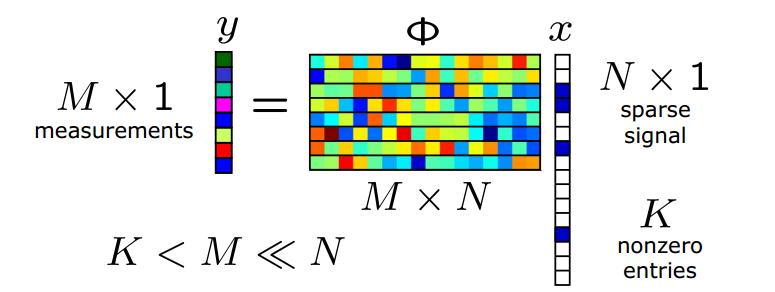
\includegraphics[height = 7 cm, width=\textwidth]{compressive_sensing_example.jpg}
\caption{A visualisation of the Compressive Sensing problem as an under-determined system}
\label{l1l2}
\end{figure*}

We may not be able to directly obtain these coefficients \(x\), as we may not posses an appropriate measuring device or one may not exist, or there is considerable uncertainty about where the non-zero coefficients are. 

Given a signal \(\alpha \in \re^n\), a matrix \(A \in \re^{m \times n}\), with \(m \ll n\),  we can acquire the signal via the set of linear measurements:

\begin{equation}
y = \Psi \alpha = \Psi\Phi x = Ax
\end{equation}
\label{cs-model}

where we have combined \eqref{vector-repr}, and \eqref{def:alpha}. In this case \(A\) represents the sampling system (i.e each column of \(A\) is the product of \(\Phi\), with the columns of \(\Psi\)). We can work with the abstract model \eqref{cs-model}, bearing in mind that \(x\) may be the coefficient seqeunce of the object in the proper basis.

In contrast to classical sensing, which requires that \(m = n\) for there to be no loss of information, it is possible to reconstruct \(x\) from an under-determined set of measurements as long as \(x\) is sparse in some basis. 

There are two conditions the matrix \(A\) needs to satisfy for recovery below Nyquist rates:

\begin{enumerate}
\item Restricted Isometry Property.
\item Incoherence between sensing and signal bases.
\end{enumerate}

\begin{definition}[RIP]\label{def:RIP}
We say that a matrix \(A\) satisfies the RIP of order \(s\) if there exists a \(\delta \in \left(0, 1\right)\) such that for all \(x \in \Sigma_s\):

\begin{equation}
\left(1 - \delta\right) \vectornorm{x}_2^2 \leq \vectornorm{Ax}_2^2 \leq \left(1 + \delta\right) \vectornorm{x}_2^2
\end{equation}
i.e. \(A\) approximately preserves the lengths of all \(s\)-sparse vectors in \(\re^n\). 
\label{def:RIP}
\end{definition}

\begin{remark}
Although the matrix \(A\) is not square, the RIP (\ref{def:RIP}) ensures that \(A^TA\) is close to the identity, and so \(A\) behaves approximately as if it were orthogonal. This is formalised in the following lemma from \cite{shalev2014understanding}:

\begin{lemma}
Let A be a matrix which satisfies the RIP of order 2\(s\) with RIP constant \(\delta\). Then for two disjoint subsets \(I, J \subset \left[n\right]\) each of size at most \(s\), and for any vector \(u \in \re^n\):

\begin{equation}
\langle Au_I, Au_J \rangle \leq \delta \vectornorm{u_I}_2 \vectornorm{u_J}_2
\end{equation}
\\
where \(u_I\) is the vector with component \(u_i\) if \(i \in I\) and zero elsewhere.

\end{lemma}

\end{remark}

\begin{remark} [Information Preservation]
A necessary condition to recover all \(s\)-sparse vectors from the measurements \(Ax\) is that \(Ax_1 \neq Ax_2\) for any pair \( x_1 \neq x_2\), \(x_1, x_2 \in \Sigma_s\), which is equivalent to \(\vectornorm{A\left(x_1 - x_2\right)}_2^2 > 0\). 

This is guaranteed as long as \(A\) satisfies the RIP of order 2\(s\) with constant \(\delta\) - as the vector \(x_1 - x_2\) will have at most \(2s\) non-zero entries, and so will be distinguishable after multiplication with \(A\). To complete the argument take \(x = x_1 - x_2\) in definition \ref{def:RIP}, guaranteeing \(\vectornorm{A\left(x_1 - x_2\right)}_2^2 > 0 \), and requiring the RIP order of \(A\) to be \(2s\).
\end{remark}

\begin{remark} [Stability]
We also require that the dimensionality reduction of compressed sensing is the preservation of relative distances: that is if \(x_1\) and \(x_2\) are far apart in \(\re^n\) then their projections \(Ax_1\) and \(Ax_2\) are far apart in \(\re^m\). This will guarantee that the dimensionality reduction is robust to noise. 
\end{remark}

A requirement on the matrix \(A\) that satisfies both of these conditions is the following:

\begin{definition}[\(\delta\)-stable embedding]
We say that a mapping is a \(\delta\)-stable embedding of \(U,V \subset \re^n\) if

\begin{equation}
\left(1 - \delta \right) \vectornorm{u-v}_2^2 \leq \vectornorm{Au-Av}_2^2 \leq \left(1 + \delta\right) \vectornorm{u-v}_2^2
\end{equation}

for all \(u \in U\) and \(v \in V\). 
\label{def:d-stable}
\end{definition} 

\begin{remark}
Note that a matrix \(A\), satisfying the RIP of order \(2s\) is a \(\delta\)-stable embedding of \(\Sigma_s, \Sigma_s\). 
\end{remark}

\begin{remark}
Definition \ref{def:d-stable} has a simple interpretation: the matrix \(A\) must approximately preserve Euclidean distances between all points in the signal model \(\Sigma_s\).
\end{remark}

\section{Incoherence}
Given that we know a basis in which our signal is sparse, \(\phi\), how do we choose \(\psi\), so that we can accomplish this sensing task? In classical sensing, we choose \(\psi_k\) to be the set of \( T_s \)-spaced delta functions (or equivalently the set of \( 1/T_s \) spaced delta functions in the frequency domain). A simple set of \(\psi_k\) would be to choose a (random) subset of the delta functions above.

In general, we seek waveforms in which the signals' representation would be dense.

\begin{definition}[Incoherence]
A pair of bases is said to be incoherent if the largest projection of two elements between the sensing (\(\psi\)) and representation (\(\phi\)) basis  is in the set \( [1 , \sqrt{n}] \), where \( n \) is the dimension of the signal. The coherence of a set of bases is denoted by \(\mu\).
\end{definition}

Examples of pairs of incoherent bases are:

\begin{itemize}
\item Time and Fourier bases: Let \(\Phi = \textbf{I}_n\) be the canonical basis and \(\Psi = \textbf{F}\) with \(\psi_i = n^{-\frac{1}{2}}e^{i\omega k} \) be the Fourier basis, then \(\mu\left(\phi, \psi\right) = 1\). This corresponds to the classical sampling strategy in time or space.
\item Consider the basis \(\Phi\) to have only entries in a single row, then the coherence between \(\Phi\) and any fixed basis \(\Psi\) will be \(\sqrt{n}\).
\item Random matrices are incoherent with any fixed basis \(\Psi\). We can choose \(\Phi\) by creating \(n\) orthonormal vectors from \(n\) vectors sampled independently and uniformly on the unit sphere. With high probability \(\mu = \sqrt{n\log{n}}\). This extends to matrices whose rows are created by sampling independent Gaussian or Bernoulli random vectors.
\end{itemize}

This implies that sensing with incoherent systems is good (in the sine wave example above it would be better to sample randomly in the time domain as opposed to the frequency domain), and efficient mechanisms ought to acquire correlations with random waveforms (e.g. white noise).

\begin{theorem}[Reconstruction from Compressive measurements \cite{Candes2006}] 
Fix a signal \(f\in \mathbb{R}^n\) with a sparse coefficient basis, \(x_{i}\) in \(\phi\). Then a reconstruction from \(m\) random measurements in \(\psi\) is possible with probability \(1 - \delta\) if: 

\begin{equation}
m \geq C \mu^2(\phi, \psi) S \log\left(\frac{n}{\delta}\right)
\end{equation}
\label{minsamples}

where \( \mu(\phi, \psi)\) is the coherence of the two bases, and \(S\) is the number of non-zero entries on the support of the signal.
\end{theorem}

\subsection{Random Matrix Constructions} \label{sec:mtx-contruction}

To construct matrices satisfying definition \ref{def:d-stable}, given \(m, n\) we generate \(A\) by \(A_{ij}\) being i.i.d random variables from distributions with the following conditions \cite{davenport2010signal}

\begin{condition}[Norm preservation]
\(\ep A_{ij}^2 = \frac{1}{m}\)
\label{cond:norm-pres}
\end{condition}

\begin{condition}[sub-Gaussian]
\(\ep\left( e^{A_{ij}t} \right) \leq e^{C^2 t^2 /2}\)
\label{cond:sub-Gauss}
\end{condition}

Random variables \(A_{ij}\) satisfying conditions \eqref{cond:norm-pres} and \eqref{cond:sub-Gauss} satisfy the following concentration inequality \cite{baraniuk2008simple}:

\begin{lemma}[sub-Gaussian]
\begin{equation}
\pr\Big( \biggl\lvert \vectornorm{Ax}_2^2 - \vectornorm{x}_2^2 \biggr\rvert\geq \varepsilon  \vectornorm{x}_2^2 \Big) \leq 2e^{-cM\varepsilon^2}
\label{cond:sub-Gauss concetration}
\end{equation} 
\end{lemma}

Then in \cite{baraniuk2008simple} the following theorem is proved:

\begin{theorem}
Suppose that \(m\), \(n\) and \(0 < \delta < 1\) are given. If the probability distribution generating \(A\) satisfies condition \eqref{cond:sub-Gauss concentration}, then there exist constants \(c_1, c_2\) depending only on \(\delta\) such that the RIP \eqref{def:RIP} holds for \(A\) with the prescribed \(\delta\) and any  \(s \leq \frac{c_1 n}{\log{n/s}}\) with probability \(\geq 1-2e^{-c_2n}\) 
\end{theorem}

For example, if we take \(A_{ij} \sim \mathcal{N}\left(0, 1/m\right)\), then the matrix \(A\) will satisfy the RIP, with probability \cite{baraniuk2008simple}

\begin{equation}
\geq 1-2\left(\frac{12}{\delta}\right)^k e^{-c_0\frac{\delta}{2}n}
\end{equation}

where \(\delta\) is the RIP constant, and \(c_0\) is a constant/

\subsection{Wishart Matrices}

Let \(\{X_i\}_{i=1}^r\) be a set of i.i.d \(1 \times p\) random vectors drawn from the multivariate normal distribution with mean 0 and covariance matrix \(H\).

\begin{equation}
X_i = \left(x_1^{(i)}, \ldots , x_p^{(i)}\right) \sim N\left(0, H\right)
\end{equation}

We form the matrix \(X\) by concatenating the \(r\) random vectors into a \(r \times p\) matrix.

\begin{definition}[Wishart Matrix]
Let 

\begin{equation}
W = \sum_{j=1}^r X_j X_j^T =  X X^T
\end{equation}

Then \(W \in \re^{r \times r}\) has the Wishart distribution with parameters 

\begin{equation}
W_r\left(H, p\right)
\end{equation}

where \(p\) is the number of degrees of freedom.
\end{definition}

\begin{remark}
This distribution is a generalisation of the Chi-squared distribution: let \(p = H = 1\). 
\end{remark}

\begin{theorem}[Expected Value]
\begin{equation}
\ep\left(W\right) = rH
\end{equation}
\end{theorem}
\begin{proof}
\begin{align*}
\ep\left(W\right) &= \ep\left(\sum_{j=1}^r X_j X_j^T\right) \\
&= \sum_{j=1}^r \ep\left(X_jX_j^T\right) \\
&= \sum_{j=1}^r \left( \mathrm{Var}(X_j) + \ep(X_j) \ep(X_j^T)   \right) \\
&= rH 
\end{align*}
Where the last line follows as \(X_j\) is drawn from a distribution with zero mean.
\end{proof}

\begin{remark}
The matrix \(M = A^TA\), where \(A\) is constructed by the methods from section \ref{sec:mtx-contruction}, will have a Wishart distribution. In particular, it will have \(\ep M = \frac{1}{m}I_n\) 
\label{remark: exp AtA}
\end{remark}

The joint distribution of the eigenvalues is given by \cite{levequeMatrices}:

\begin{equation}
p\left(\lambda_1, \ldots, \lambda_r\right) = c_r \prod_{i=1}^r e^{-\lambda_i}\prod_{i<j}\left(\lambda_i - \lambda_j\right)^2
\end{equation}

The eigenvectors are uniform on the unit sphere in \(\re^{r}\).

\section{Reconstruction Objectives}
Compressive sensing places the computational load on reconstructing the coefficient sequnce \(x\), from the set of compressive samples \(y\). This is in contrast to Nyquist sampling, where the bottleneck is in obtaining the samples themselves - reconstructing the signal is a relatively simple task. 

Many recovery algorithms have been proposed, and all are based upon minimising some functional of the data. This objective is based upon two terms: a data fidelity term, minimising the discrepancy between the reconstructed and true signal, and a regularisation term - biasing the reconstruction towards a class of solutions with desirable properties, for example sparsity. Typically the squared error \( \frac{1}{2}\vectornorm{y-Ax}_2^2 \) is chosen as the data fidelity term, whilst a number of regularisation terms have been introduced in the literature. 

A particularly important functional is:

\begin{equation}
\argmin_x \vectornorm{x}_1 \text{ s.t } y=Ax
\label{program:bp}
\end{equation}

known as Basis Pursuit \cite{Chen1998a}, with the following program known as the LASSO \cite{tibshirani1996regression} as a noisy generalisation: 

\begin{equation}
\argmin_x \frac{1}{2}\vectornorm{Ax-y}_2^2 + \lambda\vectornorm{x}_1
\label{program:lasso}
\end{equation}

The statistical properties of LASSO have been well studied. The program performs, both regularisation and variable selection: the parameter \(\lambda\) trades off data fidelity and sparsity with higher values of \(\lambda\) leading to sparser solutions. 

The LASSO shares several features with Ridge regression \cite{hoerl1970ridge}:

\begin{equation}
\argmin_x \frac{1}{2}\vectornorm{Ax-y}_2^2 + \lambda\vectornorm{x}_2^2
\label{program:Ridge-regression}
\end{equation}

and the Non-negative garrote \cite{breiman1995better} used for best subset regression:

\begin{equation}
\argmin_x \frac{1}{2}\vectornorm{Ax-y}_2^2 + \lambda\vectornorm{x}_0
\label{program:ell0}
\end{equation}

The solutions to these programs can all be related to each other - it can be shown \cite{hastie2005elements}, that the solution to \eqref{program:lasso} can be written as:

\begin{equation}
\hat{x} = S_{\lambda}\left(x^{OLS}\right) = x^{OLS} \mathrm{sign}\left(x_i - \lambda\right)
\label{soln:lasso}
\end{equation} 

where \(x^{OLS} = (A^TA)^{-1}A^Ty \) is the ordinary least squares solution, whereas the solution to Ridge regression can be written as:

\begin{equation}
\hat{x} = \left(1+\lambda\right)^{-1}x^{OLS}
\label{soln:ridge}
\end{equation}

and the solution to the best subset regression \eqref{program:ell0} where \( \vectornorm{x}_0 = \{ |i| : x_i \neq 0 \} \), can be written as:

\begin{equation}
\hat{x} = H_{\lambda}\left(x^{OLS}\right) = x^{OLS} \mathbb{I}\left(|x^{OLS}| > \lambda\right)
\label{soln:l0}
\end{equation} 

where \(\mathbb{I}\) is the indicator function. From \eqref{soln:l0} and \eqref{soln:ridge}, we can see that the solution to \eqref{program:lasso}, \eqref{soln:lasso}, translates coefficients towards zero by a constant factor, and set coefficients to zero if they are too small; thus the LASSO is able to perform both model selection (choosing relevant covariates) and regularisation (shrinking model coefficients). 

\begin{example}[Unitary A \cite{Elad2010}]


\end{example}

\begin{figure*}[h]
\centering
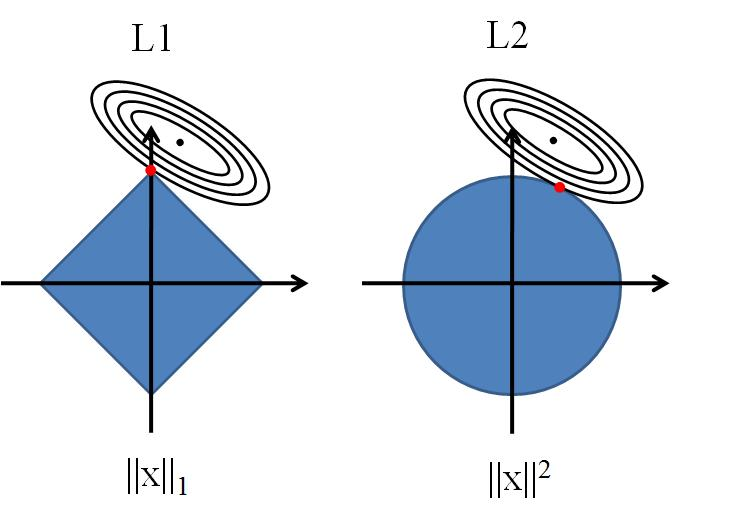
\includegraphics[height = 7 cm]{l1l2.jpg}
\caption{Solutions to the Compressive Sensing optimisation problem intersect the \(l_1\) norm the points where all components (but one) of the vector are zero (i.e. it is sparsity promoting) \cite{Tibshirani1996}}
\label{fig:l1l2}
\end{figure*}

Figure \ref{fig:l1l2}, provides a graphical demonstration of why the LASSO promotes sparse solutions. \eqref{program:lasso} can also be thought of as the best convex approximation of the \(\ell_0\) problem \eqref{program:ell0}, as the \(\ell_1\)-norm is the convex hull of the points defined by \(\vectornorm{x}_p\) for \(p < 1\) as \(p \rightarrow 0\). 

Other examples of regularisers are:

\begin{itemize}
\item Elastic Net: This estimator is a blend of both \eqref{program:lasso} and \eqref{program:Ridge-regression}, found by minimising:

\begin{equation}
\argmin_x \frac{1}{2}\vectornorm{Ax-y}_2^2 + \lambda\vectornorm{x}_2^2 + \mu\vectornorm{x}_1
\label{program:enat}
\end{equation}

The estimate has the benefits of both Ridge and Lasso regression: feature selection from the LASSO, and regularisation for numerical stability (useful in the under-determined case we consider here) from Ridge regression. The Elastic Net will outperform the LASSO (\cite{zou2005regularization}) when there is a high degree of collfinearity between coefficients of the true solution.

\item TV regularisation

\begin{equation}
\argmin_x \frac{1}{2}\vectornorm{Ax-y}_2^2 +  \lambda\vectornorm{\nabla x}_1
\label{program:enat}
\end{equation}

This type of regularisation is used when preserving edges whilst simultaneously de-noising a signal is required. It is used extensively in image processing, where signals exhibit large flat patches alongside large discontinuities between groups of pixels.

\item Candes and Tao in \cite{candes2007dantzig}, propose an alternative  functional:

\begin{equation}
\min_{x \in \re^n} \vectornorm{x}_1 \text{ s.t. } \vectornorm{A^T(Ax-y)}_{\infty} \leq t\sigma
\end{equation}

with \(t = c\sqrt{2\log{n}}\). Similarly to the LASSO this functional selects sparse vectors consistent with the data, in the sense that the residual \(r = y - Ax\) is smaller than the maximum amount of noise present. In \cite{candes2007dantzig} it was shown that the \(l_2\) error of the solution is within a factor of \(\log{n}\) of the ideal \(l_2\) error. More recent work by Bikel, Ritov, and Tsybakov, \cite{bickel2009simultaneous}, has shown that the LASSO enjoys similar properties.
\end{itemize}

%Convex algorithms all relax the \(l\)-0 requirement for recovery \cite{tropp2006relax}, by instead solving the equivalent \(l\)-1 minimisation problem:%

\section{Reconstruction Algorithms}
Broadly reconstruction algorithms fall into three classes: convex-optimisation/linear programming, greedy algorithms, and Bayesian inference. Convex optimisation methods offer better performance, measured in terms of reconstruction accuracy, at the cost of greater computational complexity. Greedy methods are relatively simpler, but don't have the reconstruction guarantees of convex algorithms. Bayesian methods offer the best reconstruction guarantees, as well as uncertainty estimates about the quality of reconstruction, but come with considerable computational complexity.

\begin{tabular}{ |p{3cm}||p{3cm}|p{3cm}|p{3cm}|  }
 \hline
 \multicolumn{4}{|c|}{Recovery Algorithm Summary} \\
 \hline
 Algorithm Type & Accuracy & Complexity & Speed\\
 \hline
 Greedy   & Low    &LowG&   Fast\\
 Convex&   Medium  & MediumA   &Medium\\
 Bayesian& High & HighB&  Slow\\
 \hline
\end{tabular}



\subsection{Convex Algorithms}
Convex methods cast the optimisation objective either as a linear program with linear constraints, or as a second order cone program with quadratic constraints. Both of these types of program can be solved with first order interior point methods. However, their practical application to compressive sensing problems is limited due to their polynomial dependence upon the signal dimension and the number of constraints. 

Compressive Sensing poses a few difficulties for convex optimisation based methods. In particular, many of the unconstrained objectives are non-smooth: meaning methods based upon descent down a smooth gradient are inapplicable. 

To overcome these difficulties, a series of algorithms originally proposed for wavelet-based image de-noising have been applied to CS, known as iterative shrinkage methods. These have the desirable property that they boil down to matrix-vector multiplications and component-wise thresholding.

Iterative shrinkage algorithms replace searching for a minimal facet of a complex polytope by a iteratively denoised gradient descent. The choice of the (component-wise) denoiser is dependent upon the regulaiser used in \ref{program:lasso}. These algorithms have an interpretation as Expectation-Maximisation \cite{figueiredo2003algorithm} - where the E-step is performed as gradient descent, and the M-step is the application of the denoiser.

\begin{figure}
\begin{algorithmic}[1]
\Procedure{IST}{$y,A, \mu, \tau, \varepsilon$}
\State $x^0 = 0$
\While{$\vectornorm{x^{t} - x^{t-1}}_2^2 \leq \varepsilon$}
\State $x^{t+1} \gets S_{\mu\tau}\left(x^t + \tau A^Tz^t \right) $
\State $z^t \gets y - Ax^t$
\EndWhile
\State \textbf{return} $x^{t+1}$
\EndProcedure
\end{algorithmic}
\caption{The Iterative Soft Thresholding Algorithm}\label{alg:IST}
\end{figure}

There has been a line of work on algorithms directly minimising the \(\ell_0\) norm \cite{wen2015efficient}, \cite{oxvig2012improving}, \cite{mohimani2010sparse}. Even though this objective function is no longer convex, the proximity operator (see definition \eqref{def:prox_operator}) the \(\ell_0\)-norm can be computed, and so this minimisation can be cast as shrunk gradient descent. Thus the direct inverse problem for CS can be solved exactly, and efficiently.

\subsection{Greedy Algorithms}
Greedy methods are another family of solutions to \ref{program:lasso}. They offer reduced computational complexity with correspondingly worse reconstruction quality and poorer guarantees on sparsity and undersampling than convex algorithms. Examples of this type are Orthogonal Matching Pursuit (OMP)\cite{tropp2007signal}, Subspace Pursuit \cite{dai2009subspace}, and Compressive Sensing Orthogonal Matching Pursuit (CoSaMP).

\begin{figure}
\begin{algorithmic}[1]
\Procedure{OMP}{$y,A,K,\varepsilon$}
\State $x^0 = 0$, $r=y$, $\Omega = \varnothing$, $i=0$
\While{$\vectornorm{x^{t} - x^{t-1}}_2^2 \leq \varepsilon$}
\State $i \gets i+1$
\State $b\gets A^Tr$
\State $\Omega \gets \Omega \cup \mathrm{supp}\left(H_1\left(b\right)\right)$
\State $x\restriction_{\Omega} \gets A^T\restriction_{\Omega}x$
\State $x\restriction_{\Omega^c} \gets 0$
\State $b \gets y - A\restriction_{\Omega} A^T\restriction_{\Omega}x$
\EndWhile
\State \textbf{return} $x$
\EndProcedure
\end{algorithmic}
\caption{The OMP recovery algorithm}\label{alg:omp}
\end{figure}


\begin{figure*}[h]
\centering
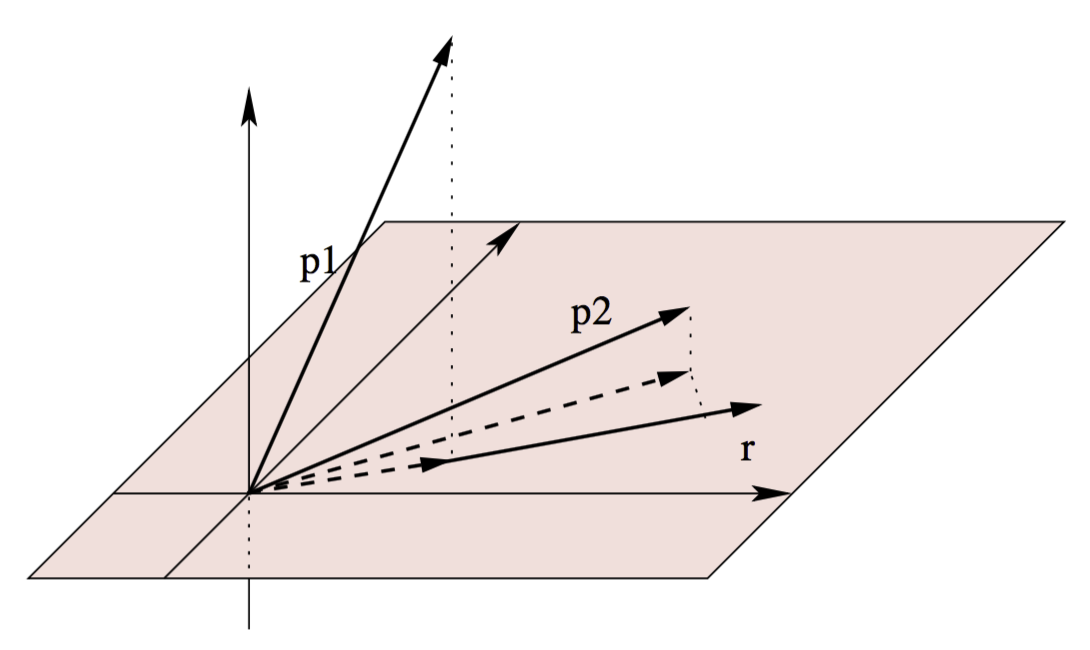
\includegraphics[height = 7 cm]{OMP_illustration.png}
\caption{An illustration of the orthognalisation step of OMP. \cite{blumensath2007difference}}
\label{fig:OMP}
\end{figure*}

Greedy pursuit algorithms abandon exhaustive searches of the solution space in favour of locally optimal single term updates. Representative of this type of algorithm is Orthogonal Matching Pursuit (OMP), which proceeds by approximating the solution by some active set of columns from the sensing matrix \(A\). In detail the algorithm finding the index of the largest remaining element not in the support set via matched filtering and (hard) thresholding. Then a residual in the orthogonal complement of the space spanned by the current active set is computed. This guarantees a maximal reduction in \(l\)-2 error in each iteration.

These ideas are illustrated in in figure \eqref{fig:OMP}. Assuming the previous signal approximation is along the vertical axis, the residual from the current step will be in the subspace orthogonal to this direction (the pink plane) - labelled \(r\). The elements of \(A\) which have not been selected do not have to lie in this subspace - they are illustrated as \(p_1\) and \(p_2\). OMP selects the largest element of \(A\) not currently included, with the largest inner product with the current residual. In the figure this is \(p_2\).

OMP has a long history in statistics and signal processing. It was first introduced in the statistics literature as stepwise least squares \cite{goldberger1961stepwise}, and proposed by Pati et al in \cite{pati1993orthogonal} as a modification of the Matching Pursuit algorithm of Mallet and Zhang \cite{mallat1993matching} maintaining full backward orthogonality of the residual. The use of OMP for solving Compressive Sensing problems was studied by Tropp and Gilbert in \cite{tropp2007signal}. 

Subspace pursuit and CoSaMP are matching pursuit algorithms specifically designed for compressive sensing problems. The main difference between these and OMP, is that they compute the \(T\) largest components in the matched filtering stage along with solving a least-squares problem to with the selected indices to identify the new support set.

Despite their computational simplicity, greedy algorithms have several drawbacks. Primarily they do not come with stable recovery guarantees, and they require a larger number of samples to recover the signal when compared to Bayesian and Convex recovery algorithms. Also, due to their greedy nature, these algorithms are not guaranteed to converge: in fact it was shown in \cite{wen2013improved} that there exist \(k\)-sparse vectors and sensing matrices \(A\) such that OMP fails to converge in k iterations.

\begin{figure}
\begin{algorithmic}[1]
\Procedure{AMP}{$y,A,\varepsilon$}
\State $x^0 = 0$, $z^0=A^Ty$
\While{$\vectornorm{x^{t} - x^{t-1}}_2^2 \leq \varepsilon$}
\State $x^{t+1} \gets S_{\mu\tau}\left(x^t - \tau+ A^Tz^t\right) $
\State $z^{t+1} \gets y - Ax^t + \frac{\vectornorm{x}_0}{m}z^t$
\EndWhile
\State \textbf{return} $x^{t+1}$
\EndProcedure
\end{algorithmic}
\caption{The AMP recovery algorithm}\label{alg:amp}
\end{figure}

\subsection{Bayesian Algorithms}
Bayesian methods reformulate the optimisation problem into an inference problem. These methods come with a unified theory, and standard methods to produce solutions. The theory is able to handle hyper-parameters in a elegant way, provides a flexible modelling framework, and is able to provide desirable statistical quantities such as the uncertainty inherent in the prediction.

Previous sections have discussed how the weights \(x\) may be found through optimisation methods such as basis pursuit or greedy algorithms. Here, an alternative Bayesian model is described.

Equation \eqref{CSequation} implies that we have a Gaussian likelihood model: 

\begin{equation}
p \left(y \mid z\text{,} \sigma^2 \right) = (2 \pi \sigma^2)^{-K/2} \exp{\left(- \frac{1}{2 \sigma^2} \|y - Ax|_{2}^{2} \right)} 
\end{equation}

The above has converted the CS problem of inverting sparse weight \textbf{w} into a linear regression problem with a constraint (prior) that \textbf{w} is sparse. 

To seek the full posterior distribution over \textbf{w} and \( \sigma^2 \), we can chose a sparsity promoting prior. A popular sparseness prior is the Laplace density functions:

\begin{equation}
p\left(x\mid\lambda\right) = \left(\frac{\lambda}{2}\right)^N \exp{-\lambda \sum_{i=1}^{N} |x_i|}
\end{equation}

Note that the solution the convex optimisation problem \eqref{program:lasso} corresponds to a maximum \textit{a posteriori} estimate for \(x\) using this prior. I.e this prior is equivalent to using the \(l_1\) norm as an optimisation function (see figure \ref{laplacenormal} \cite{Tibshirani1996}).

\begin{figure*}[h]
\centering
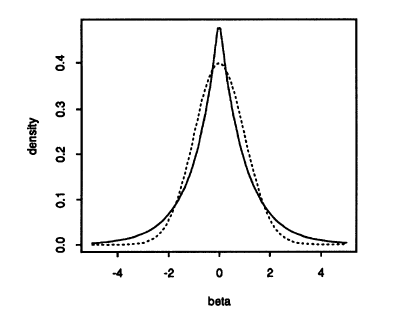
\includegraphics[height = 7 cm]{LaplaceandNormalDensity.png}
\caption{The Laplace (\(l_1\)-norm, bold line) and Normal (\(l_2\)-norm, dotted line) densities. Note that the Laplace density is sparsity promoting as it penalises solutions away from zero more than the Gaussian density. \cite{Tibshirani1996}}
\label{laplacenormal}
\end{figure*}

The full posterior distribution on \(x\) and \(\sigma^2\) may be realised, by using a hierarchical prior instead. To do this, define a zero-mean Gaussian prior on each element of \(n\):
%
\begin{equation}
p\left(n\mid a\right) = \prod_{i=1}^{N}\mathbb{N}\left(n_i\mid 0, \alpha_{i}^{-1}\right)
\end{equation}
%
where \(\alpha\) is the precision of the distribution. A gamma prior is then imposed on \(\alpha\):

\begin{equation}
p\left(\alpha \mid a, b \right) = \prod_{i=1}^{N} \Gamma\left( \alpha_i \mid a, b \right)
\end{equation}

The overall prior is found by marginalising over the hyperparameters:

\begin{equation}
p\left( x \mid a, b \right) = \prod_{i=1}^{N} \int_{0}^{\infty} \mathbb{N}\left(w_i\mid 0, \alpha_{i}^{-1}\right) \Gamma\left( \alpha_i \mid a, b \right)
\end{equation}

This integral can be done analytically and is a Student-t distribution. Choosing the parameters \(a,b\) appropriately we can make the Student-t distribution peak strongly around \(x_i = 0\) i.e. sparsifying. This process can be repeated for the noise variance \(\sigma^2\). The hierarchical model for this process is shown in figure \ref{fig:bayesiancs}. This model, and other CS models which not necessarily have closed form solutions, can be solved via belief-propagation \cite{Baron2010}, or via Monte-Carlo methods.

\begin{figure}[h]
\centering
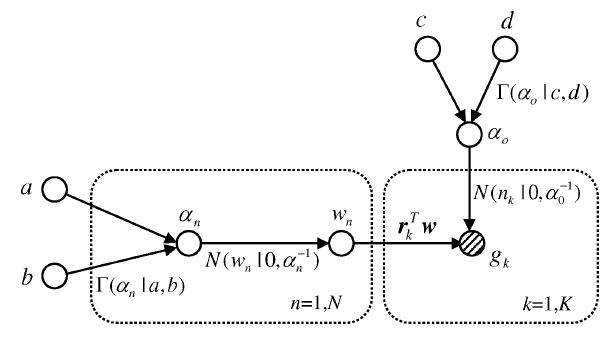
\includegraphics[height = 7 cm]{bayesiancs.png}
\caption{The hierarchical model for the Bayesian CS formulation \cite{Ji2008}}
\label{fig:bayesiancs}
\end{figure}

However, as with all methodologies, Bayesian algorithms have their drawbacks. Most notable is the use of the most computationally complex recovery algorithms. In particular MCMC methods suffer in high dimensional settings, such as those considered in compressive sensing. There has been an active line of work to address this: most notably Hamiltonian Monte Carlo (see \cite{neal2011mcmc}) - an MCMC sampling method designed to follow the typical set of the posterior density. 

Belief propagation (BP) \cite{Yedidia2011} is a popular iterative algorithm, offering improved reconstruction quality and undersampling performance. However, it is a computationally complex algorithm. It is also difficult to implement. Approximate message passing (figure \ref{alg:amp}) solves this issue by blending BP and (IT). The algorithm proceeds like iterative thresholding (figure \ref{alg:IST}), but computes an adjusted residual at each stage. The final term in the update:

\begin{equation}
z^{t+1} = y - Ax^t + \frac{\vectornorm{x}_0}{m}z^t
\end{equation}

comes from a first order approximation to the messages passed by BP \cite{metzler2014denoising}. This is in contrast to the update from IST (figure \ref{alg:IST}):

\begin{equation}
z^{t+1} = y - Ax^t
\end{equation}

The choice of prior is key in Bayesian inference, as it encodes all knowledge about the problem. Penalising the least-squares estimate  with the \(\ell_1\) norm,

\section{Compressive Sensing Architectures}\label{sec:sensingmodel}

\subsection{Modulated Wideband Converter}
We try to sense and reconstruct a wideband signal, divided into \(L\) channels. We have a (connected) network of \(J\) (= 50) nodes placed uniformly at random within the square \(  \left[0,1\right]\times \left[0,1\right] \). This is the same model, as in \cite{Zhang2011b}. The calculations which follow are taken from \cite{Zhang2011b} as well.

The nodes individually take measurements (as in \cite{mishali2010theory}) by mixing the incoming analogue signal \(x\left(t\right)\) with a mixing function \(p_i\left(t\right)\) aliasing the spectrum. \(x\left(t\right)\) is assumed to be bandlimited and composed of up to \(k\) uncorrelated transmissions over the \(L\) possible narrowband channels - i.e. the signal is \(k\)-sparse. 

\begin{figure}[h]
\centering
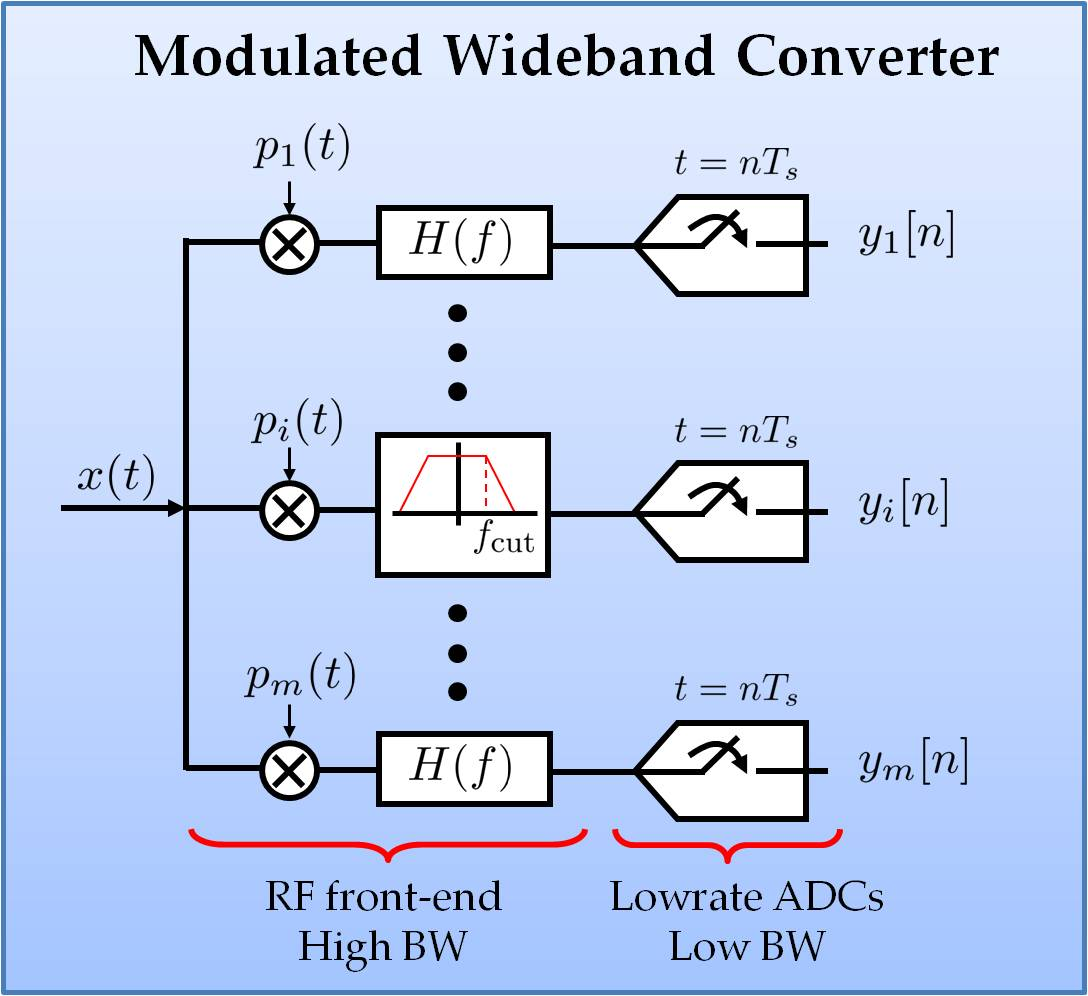
\includegraphics[height = 7.3 cm]{Modulated_wideband_converter.jpg}
\caption{Mse vs SNR for the sensing model, with AWGN only, showing the performance of distributed and centralised solvers}
\label{msevssnr0}
\end{figure}

The mixing functions - which are independent for each node - are required to be periodic, with period \(T_p\). Since \(p_i\) is periodic it has Fourier expansion:

\begin{equation}
p_i\left(t\right) = \sum_{l=-\infty}^{\infty} c_{il} \exp\left({jlt\frac{2\pi}{T_p}}\right)
\end{equation}

The \(c_{il}\) are the Fourier coefficients of the expansion and are defined in the standard manner. The result of the mixing procedure in channel \(i\) is therefore the product \(xp_i\), with Fourier transform (we denote the Fourier Transform of \(x\) by \(X\left( \dot{.} \right)\)):

\begin{align}
X_{i}\left(f\right) &=& \int_{-\infty}^{\infty} x\left(t\right) p_i\left(t\right) dt \nonumber
\\ &=& \sum_{l=-\infty}^{\infty} c_{il} X\left(f-lf_p\right)
\end{align}

(We insert the Fourier series for \(p_i\), then exchange the sum and integral). The output of this mixing process then, is a linear combination of shifted copies of \(X\left(f\right)\), with at most \(\lceil f_NYQ/f_p\rceil\) terms since \(X\left(f\right)\) is zero outside its support (we have assumed this Nyquist frequency exists, even though we never sample at that rate).

This process is repeated in parallel at each node so that each band in \(x\) appears in baseband.

Once the mixing process has been completed the signal in each channel is low-pass filtered and sampled at a rate \(f_s \geq f_p\). In the frequency domain this is a ideal rectangle function, so the output of a single channel is:

\begin{equation}
Y_i\left(e^{j 2 \pi f T_s }\right) = \sum_{l = -L_0}^{+L_0} c_{il} X\left(f-lf_p\right)
\end{equation}

since frequencies outside of \([-f_s/2, f_s/2]\) will filtered out. \(L_0\) is the smallest integer number of non-zero contributions in \(X\left(f\right)\) over \([-f_s/2, f_s/2]\) - at most \(\lceil f_NYQ/f_p\rceil\) if we choose \(f_s = f_p\). These relations can be written in matrix form as:

\begin{equation}
\textbf{y} = \textbf{A}\textbf{x} + \vec{w}
\label{system}
\end{equation}

where \(\textbf{y}\) contains the output of the measurement process, and \(\textbf{A}\) is a product matrix of the mixing functions, their Fourier coefficients, a partial Fourier Matrix, and a matrix of channel coefficients. \(\textbf{x}\) is the vector of unknown samples of \(x\left(t\right)\). 

i.e. \(\textbf{A}\) can be written: 

\begin{equation}
\textbf{A} = \textbf{S} \textbf{F} \textbf{D} \textbf{H}
\end{equation}

The system  \ref{system} can then be solved (in the sense of finding the sparse vector \(\vec{x}\) by convex optimisation via minimising the objective function:

\begin{equation}
\frac{1}{2}\|\textbf{Ax}-\textbf{y}\|_2^2 + \lambda \|\textbf{x}\|_1
\end{equation}

where \(\lambda\) is a parameter chosen to promote sparsity. Larger \(\lambda\) means sparser \(\vec{x}\).

\subsection{Random Demodulator}
The random demodulator was introduced by Rice University in \cite{kirolos2006analog} and extended in \cite{ harms2013constrained}, where limitations were placed on the switching rate of the random waveform. The architecture consists of three main steps: demodulation, filtering, and uniform sampling. 

We assume that the analogue signal \(x\left(t\right)\) is bandlimited, periodic, and comprised of a finite number of components from some arbitrary dictionary (for example ) \(\psi_n\left(t\right)\):

\begin{equation}
x\left(t\right) = \sum_{n=1}^N \alpha_n \psi_n\left(t\right)
\end{equation}

Initially, the signal is modulated by a pseudo-random sequence \(p_c\left(t\right)\), which alternates at frequencies at (or above) the Nyquist frequency of \(x\left(t\right)\). As \(x\) is multitoned, the chipping sequence will spread the tones across the entire spectrum. The signal is then filtered - this filter acts as an accumulator and sums the demodulated signal, before being sampled at rate \(\mathcal{M}\) with a traditional ADC.

The output of this system, \(y\left[m\right]\), can be related to the input \(x\left(t\right)\) via a linear transformation of the coefficient vector \(\alpha_n\). 

To find the transformation \(A\), first consider the output \(y\left[m\right]\), which is the result of convolution and demodulation followed by sampling at rate \(\mathcal{M}\):

\begin{equation}
y\left[m\right] = \int_{-\infty}^{\infty} x\left(\tau\right)p_c\left(\tau\right)h\left(t - \tau\right)d\tau\mid_{t = m\mathcal{M}}
\end{equation}

and by expanding \(x\left(t\right) = \sum_{n=1}^N \alpha_n \psi_n\left(t\right)\):

\begin{equation}
y\left[m\right] =  \sum_{n=1}^N \alpha_n \int_{-\infty}^{\infty} \psi_n\left(t\right)p_c\left(\tau\right)h\left(m\mathcal{M} - \tau\right)d\tau
\end{equation}

we see that the output can be written as:

\begin{equation}
y = Ax
\end{equation}

with

\begin{equation}
A_{m,n} = \int_{-\infty}^{\infty} \psi_n\left(t\right)p_c\left(\tau\right)h\left(m\mathcal{M} - \tau\right)d\tau
\end{equation}

This random demodulation process ensures that each tone in the signal is identifiable in the filter's passband, and because there are few tones present in the signal they are identifiable from the low rate samples. 

An extension of the Random Demodulator is the Random Modulation Pre-Integrator (RMPI). This device was introduced in \cite{yoo2012design} and is an universal compressive sensing apparatus. It is a variant of the Random Demodulator, but one which uses multiple channels. 

The RMPI works by modulating the input signal by a different pseudo-random sequence per channel, where the random sequences oscillate at the Nyquist rate. Then the output of each modulator is integrated over a time period \(T\) chosen to be as large as possible (to lower the sampling rate), whilst still allowing fast computation. 

\begin{figure*}[h]
\centering
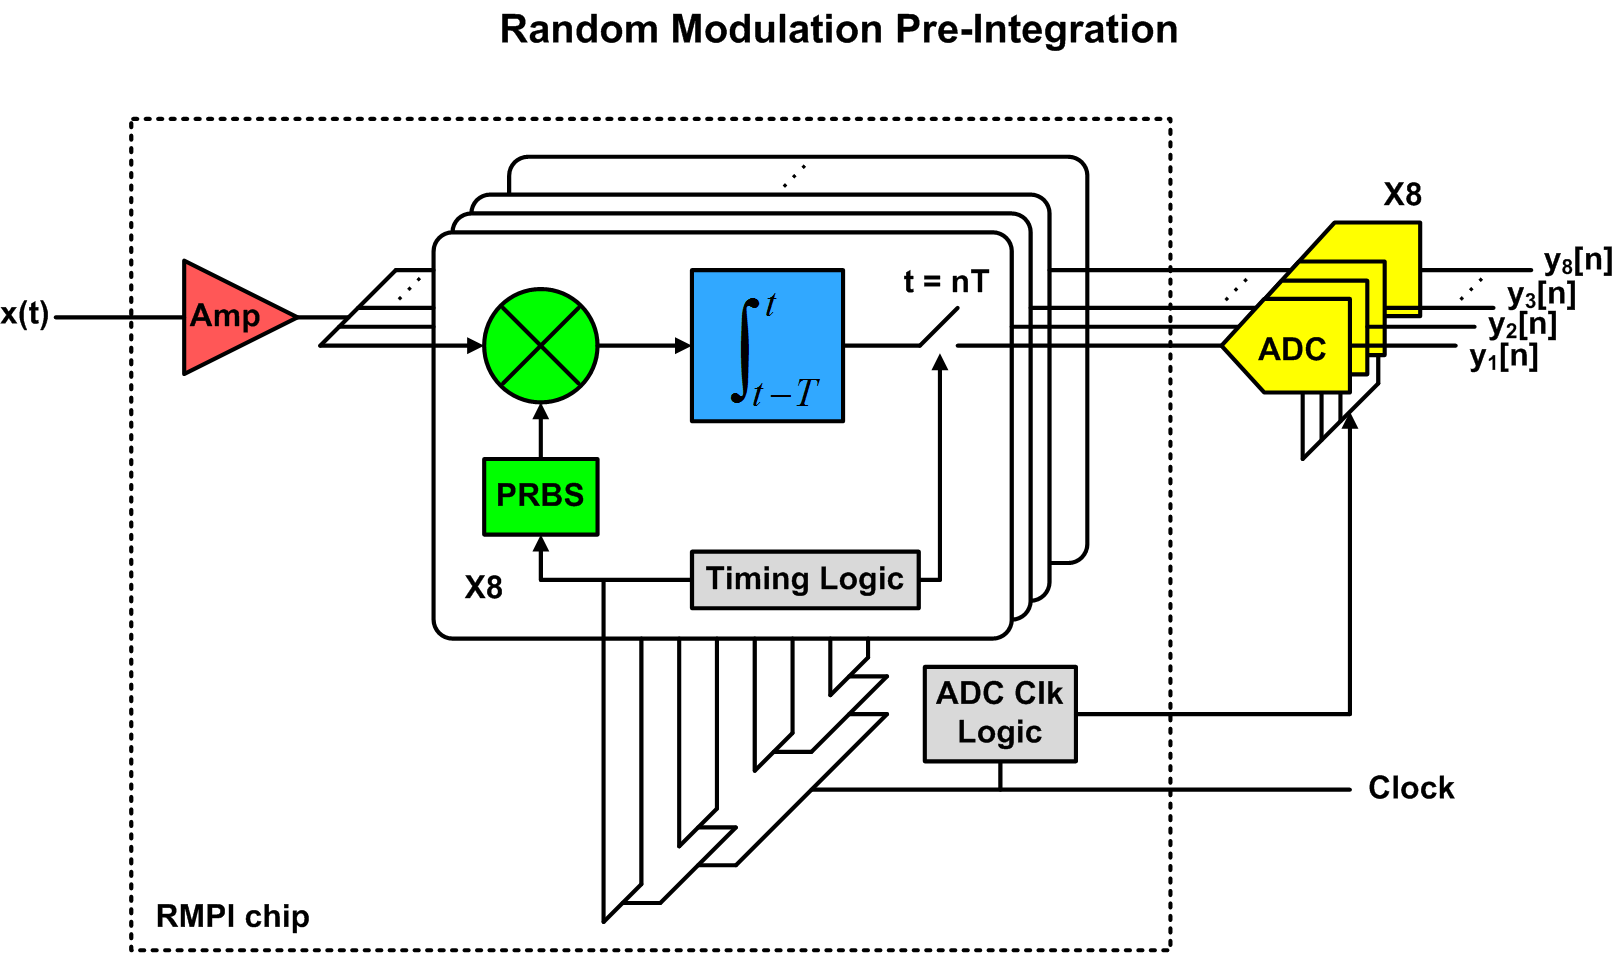
\includegraphics[height = 7 cm]{RMPI.png}
\caption{The hierarchical model for the Bayesian CS formulation \cite{Ji2008}}
\label{bayesiancs}
\end{figure*}

The main innovation in the RMPI when compared to the Random Demodulator is that it is much easier to mix the signal at the Nyquist rate, than it is to sample at the Nyquist rate. This allows the RMPI to reduce the sampling rate by a factor of \(n\), (where \(n >> gg\), a much larger factor than the Random Demodulator. 

There are several drawbacks to the Random Demodulator, which are not addressed by either the RMPI or the Modulated Wideband Converter. In particular, they are the need to generate a random chipping sequence, and high complexity from using multiple channels in the RMPI and MWC. The high rate chipping sequence used in the RD and RMPI results in high power consumption, and drains battery life of the device. This issue has been addressed in \cite{massoud2011efficient}, which proposes using frequency division multiplexing to generate the random sequences. Parallel realisations of the Random Multiplexer further increase the power drain, complexity and cost by each parallel channel employing a high rate mixer, and a relatively low rate ADC. 

There is at least one other disadvantage to the RD: circuit realisations of the RD cannot have a chipping sequence which switches at infinite polarity - it is difficult to practically generate a fast switching random sequence. To address this issue Harms et al in  \cite{harms2013constrained} modify the RD to use random waveforms with constraints on the switching rate - specifically, fully random waveforms are replaced with Run Length Limited sequences. Harms et al demonstrate that by choosing the signal statistics correctly - specifically the power spectrum of the chipping sequence should match the power spectrum of the tones to be sensed for the performance of the constrained random demodulator will match that of the random demodulator. Whether this can be achieved in practice is an open question. 

\subsection{Compressive Multiplexer}
Slivinsky et al in \cite{Slavinsky2011}, introduced the compressive multiplexer. This architecture assumes the signal is divided into multiple discontiguous channels, whose occupancy is collectively sparse. The Compressive Multiplexer (\gls{cmux}) acquires \(J\) independent channels, each of bandwidth \(W/2\) Hz, into a single stream running at the Nyquist rate of any single channel. 

The process is achieved by initially mixing the channels down to baseband, and then performing multiplying with a chipping sequence. Finally the spread channels are summed and sampled once per chip by a single ADC. This summation occurs across channels and not in time, in contrast to the \gls{rd}, and the \gls{mwc}.

Mathematically the \gls{cmux} can be represented as \(\Phi\) a \(W \times JW\) matrix, formed by concatenating \(J\) \(W \times W\) matrices horizontally. All elements along the diagonals are considered as Rademacher random variables. The sparsity basis of this model is the Fourier basis. In other words, the samples are acquired as:

\begin{equation}
y = Ax
\end{equation}

where 

\begin{equation}
A = \left[\Phi_1 \mathcal{F} \ldots \Phi_J \mathcal{F}\right]
\end{equation}

and \(\mathcal{F}\) is the \(W \times W\) Fourier matrix. 

\section{Compressive Sampling for Spectrum Sensing}

\subsection{Noise Folding}
In all measurement systems, there are two types of noise: measurement noise (noise caused by hardware imperfections) and signal noise (stochastic variations in the signal induced by the transmission environment). That is the received signal can be modelled as:

\begin{equation}
y = A(x+e) + w 
\end{equation}

where \(y \in \re^m\) is the received signal, \(A \in \re^{m \times n}\) is the measurement matrix, \(x \in \re^n\) is the signal, \(e \in \re^n\) is the signal noise, and \(n \in \re^m\) is the measurement noise. This is a different model compared to that presented in the rest of this section: part of the noise is now scaled by the measurement matrix \(A\). It is commonly assumed in the literature that \(e = 0\), and that \(w\) is a vector drawn from a sub-Gaussian distribution. We assume that that \(w\) is non-zero, and is drawn from an \(n\)-dimensional sub-Gaussian distribution. In \cite{davenport2012pros}, Davenport et al quantify the impact of this extra scaling. They begin by introducing the following measures of SNR:

\begin{definition}{Input SNR}
\begin{equation}
\mathrm{ISNR} = \frac{\vectornorm{x}_2^2}{\ep{\vectornorm{e\mid_\Gamma}}_2^2}
\end{equation}
where \(\Gamma\) represents the support of \(x\), and the expectation is taken with respect to the Lebesque measure.
\end{definition}

\begin{definition}[Recovered SNR]
\begin{equation}
\mathrm{RSNR} = \frac{\vectornorm{x}_2^2}{\ep{\vectornorm{\hat{x}-x}}_2^2}
\end{equation}
\end{definition}

They then show

\begin{theorem}[\cite{davenport2012pros}]
Suppose, \(y= A(x+e)\) where \(e \in \re^n\) is a zero-mean white random vector, and \(x\) is \(s\)-sparse, and \(A \in \re^{m \times n}\) satisfies the RIP (see definition \eqref{def:RIP}) with constant \(\delta\) and has orthogonal rows each with norm \(\sqrt{\rho}\). Then the RSNR of an oracle-assisted recovery algorithm satisfies:

\begin{equation}
\frac{\rho}{1+\delta} \leq \frac{\mathrm{ISNR}}{\mathrm{RSNR}} \leq \frac{\rho}{1-\delta}
\end{equation}

If the ratio of RNSR and ISNR is measured in dB, we have:

\begin{equation}
\frac{\mathrm{ISNR}}{\mathrm{RSNR}} \sim 10\log_{10}{\rho}
\end{equation}

\end{theorem}

In other words, for every doubling of the subsampling factor \(\rho\), the SNR loss increases by 3dB. This degradation is an important tradeoff in the design of CS receivers. It implies that for a signal with fixed bandwidth \(W/2\), there is a practical limit to the instantaneous bandwidth \(n/2\) for which any desired RSNR can be obtained. 

\subsection{Dynamic Range}
Because Compressive Sensing allows us to lower the sampling rate in order to sense a sparse signal, this allows the use of higher resolution ADCs. Thus a CS acquisition system, should exhibit a larger dynamic range than a conventional system. Firstly we define the signal-to-quantisation noise ratio:

\begin{definition}
\begin{equation}
\mathrm{SQNR} = \frac{\vectornorm{x}_2^2}{\vectornorm{x-\mathrm{Q}_b(x)}_2^2}
\end{equation}
where \(Q_b(x)\) is the \(b\)-bit quantised version of \(x\).
\end{definition}

Then \cite{davenport2012pros} shows that:

\begin{theorem}
Suppose \(y=Ax\), where \(x\) is \(s\)-sparse and \(A\) satisfies the RIP with constant \(\delta\). Let \(\hat{x}\) denote the output of applying a recovery algorithm to the quantised measurements \(Q_b(y)\), which satisfies:

\begin{equation}
\vectornorm{\hat{x}-x}_2^2 \leq \kappa \vectornorm{Q_b(y) - y}_2^2
\end{equation}

then,

\begin{equation}
\mathrm{RSNR} \geq \frac{\mathrm{SQNR}}{(1+\delta)\kappa}
\end{equation}
\end{theorem}



\subsection{CS models}
One of the first uses of Compressive Sensing for spectrum sensing was the work of Tian and Giannakis in \cite{Tian2007}. In this work, the authors proposed reconstructing the (discrete) gradient of the frequency spectrum. In this work the authors propose the following model:

\begin{equation}
\hat{z} = \argmin_z \vectornorm{z}_1 \text{ s.t } \left(SG\right)z = x 
\end{equation}

In this model, \(x \in \re^n\) is a discretisation of a continuous, piecewise smooth spectrum, \(S \in \re^{m \times n}\) is a sampling operator, for example a partial Fourier matrix or a random set of Nyquist measurements, and \(G \in \re^{n \times n}\) is a product matrix:

\begin{equation}
G = \left(F_n^{-1} \Phi \right)^{-1}\Gamma^{-1}
\end{equation}

where \(F_n\) is the \(n \times n\) Fourier matrix, \(\Phi\) is the inverse Wavelet matrix (for example, \(\Phi\) could be the Haar matrix), and \(\Gamma\) is the \(n \times n\) discrete derivative matrix.

We then see, that \(z\) is the derivative of the Wavelet modulus, and that frequency bands can be estimated from the peaks of \(z\). It is noted in \cite{Tian2007} that as the scale factor of the Wavelets increases, the noise variance is reduced. 

In \cite{polo2009compressive}, Polo et al improve on the methodology of \cite{Tian2007}. The main innovation from this work is that to perform the compressive sensing directly, as opposed to Tian et al, where the signal was sampled at a Nyquist rate, before compression via a random sampling operator. Polo et al replace this with an Analogue-to-Information converter. 

It has been assumed that the received signal vector in CS systems would be wide-sense stationary (WSS). However, in \cite{sundman2010use}, Sundman et al disagreed with this assumption - they interpret the sensing matrix \(A\) in CS measurements:

\begin{equation}
y = Ax
\end{equation}

where the elements of \(A\) are chosen randomly from a sub-Gaussian distribution, as a time-varying linear filter. Thus, the CS spectrum sensing system will not be a time-invariant, and the WSS property of the original signal will not necessarily be preserved by the measurement process.

The authors subvert this problem, by instead adopting a definition of the recovered signal based upon the autocorreleation matrix, instead of the autocorrelation sequence of the edge-spectrum.

More recently, a feature detection model has been proposed by Tian, Tafesse, Sadler \cite{tian2012cyclic}. The authors note that the cyclic spectrum of communication signals is sparse. The paper directly reconstructs the 2-D cyclic spectrum from the compressive samples, without reconstructing the signal as an intermediate step. This is possible because of the linear relationship between the cyclic covariance function and the cyclic spectrum (the quantities are related by a Fourier transform). Once the covariance vector of the data has been formed, the cyclic spectrum can be recovered using the LASSO. For details see \cite{tian2012cyclic}.

These ideas have been significantly extended, and now arbitrary second order statistics can be computed from compressive samples, without the original signal being reconstructed as an intermediate step. The applications include, wideband spectrum sensing, incoherent imaging, and power spectrum estimation. The manuscript \cite{romero2016compressive} has more details. In particular the framework is extended to array signal processing, and to source localistaion problems in radar.

In \cite{havary2010compressive} Havary and Valaee propose a bank of filters, far less in  number than the number of channels in a frequency spectrum, into which the wideband signal will be fed. The outputs of these filters are used to reconstruct the channel occupancies by comparing the results of a standard \(\ell_1\) minimisation algorithm, with a pre-defined vector of energy thresholds. Simulations shown in the paper suggest that a 20 channel signal can be accurately sensed with 12-15 filters.

Braun et al in \cite{braun2009signal} build upon this line of work, and the work of \cite{Davenport2007} and, by using a compressive matched filter (\textit{smashed filter}) for compressive detection. The authors consider the problem of detecting narrow band pilot sequences in wideband signals, comparing a smashed filter with a matched filter. The authors conclude that in an AWGN scenario, compressive sensing can be used to significantly reduce sampling rates without affecting the reliability of the detector. What is significant about this work, is that neither the signal, nor any second order statistics are reconstructed at any stage. This is in contrast to most applications of compressive sensing where some quantity of interest is reconstructed as part of the signal processing chain. These ideas were significantly extended in \cite{davenport2010signal}, which extends the ideas of \cite{Davenport2007} to estimation, and classification scenarios without an expensive reconstruction algorithm as an intermediate step.

In \cite{lexa2011compressive}, Lexa et al build upon these ideas, proposing a sub-Nyquist method for Power Spectral Density estimation for WSS signals, based upon multi-coset sampling. The authors show that the system computes an approximation to the true PSD, and that expensive \(\ell_1\) minimisation techniques need not be resorted to regardless of the sparsity of the underlying signal. 

There have also been many distributed models of wideband spectrum sensing introduced in the literature. The first detailed approach to distributed CS was by \cite{Duarte}, where the authors considered a network of nodes cooperating amongst each other to sense signals which are jointly sparse among the nodes.

The ideas of \cite{Duarte} are extended in \cite{Ma2014b}, where the authors consider ergodic signals instead of sparse signals. They establish that these signals can be sensed effectively in the compressive sensing framework.

In \citep{Zhang2011a}, the distributed Compressive Sensing framework is applied to wideband spectrum sensing via a sensor network. The authors propose a probabilistic graphical model to capture the occupancy common to all nodes, as well as spectrum occupancy viewed at a single node. That is, the authors consider the situation of a heterogeneous network where nodes are affected by different primary users, the set of which is not necessarily the same for all sensors. Belief Propagation is used to perform the statistical inference, and recover the spectrum occupancy at each node from the cooperative CS samples. Simulations indicate that this method performs wells in comparison with other methods.

Zhang et al in \cite{Zhang2011b} propose a simpler model, where a network of sensors captures a wideband signal with no innovations at any node. Their signal model is based upon the Modulated Wideband Converter \cite{Mishali2010}, but in this scenario, each node independently has a single channel of the converter. Reconstruction is done at a nominated fusion node, which has access to all the measurements taken by the network (via communication). Simulations reported by the authors suggest that the method is promising. 

These late two papers, \citep{Zhang2011a}, and \cite{Zhang2011b} both transmit the compressive measurements to a Central node, which does the requisite processing. Either via Belief Propagation as in \cite{Zhang2011a}, or via the Alternating Direction Method of Multipliers \cite{Zhang2011b}. This is a common pattern in distributed sensing, as it allows the system to gain statistical strength via spatial diversity whilst also allowing fast computation at a single node. However, this method also introduces a single point of failure: should the fusion node fail in some way (lose power, find itself in a deep fade in the radio environment etc), then the system cannot recover the original signal. This motivates the use of distributed solvers to go along with the distributed capture of frequency spectra.

An example of this kind of work is \cite{Sundman2013a}, where the distributed CS model is extended to several sparsity models, which capture differing signal intercorrelations amongst nodes. We are primarily interested in the common signal model: that is all nodes within the network observe the same sparse signal, but under differing noise and fading. The paper also develops a distributed greedy pursuit algorithm for inverting the compressive samples, based upon orthogonal matching pursuit. The authors demonstrate via extensive simulations that the distributed algorithm matches the performance of a centralised greedy algorithm. 

In \cite{schizas2008consensus}, distributed estimation of signals is analysed from a statistical point of view. Schizas et al establish that there exist algorithms with guaranteed convergence to the required estimator (for example Maximum Likelihood) in the presence of fading and noise, for sensor networks with ideal links. In particular the authors introduce a decentralised scheme for least-squares and best linear unbiased estimator (BLUE). 

The same authors build on this work in \cite{schizas2008consensus2}, and extend their analysis to decentralised MAP estimators. Again they show that when consensus is achieved between sensors, the estimate has converged to the ideal MAP estimate. In both papers, the authors express the desired estimator (either least-squares or MAP) as a convex optimisation problem over the nodes of the network, and then show that the Alternating Direction Method of Multipliers will suffice as an algorithm to compute the estimate. The framework doesn't require that the estimator be expressed in closed form and the estimation procedure is resilient to communication noise.

Finally, there has been some work on compressive detection applied to spectrum sensing. Notably in  \cite{verlant2012multiband}, and \cite{bodart2015multiband} the work of \cite{Davenport2010} is applied to cognitive radio. In the first paper, the authors